\documentclass[a4paper]{article}
\usepackage{geometry}
 \geometry{
 a4paper,
 total={210mm,297mm},
 left=1.25in,
 right=1.25in,
 top=1.25in,
 bottom=1.25in,
 }
\usepackage{graphicx}
\usepackage{pdfpages}
\usepackage{hyperref}

\begin{document}

\title{Some of my reports for Hardware and Software Projects}
\author{Sasank Chilamkurthy - 110070051}
\date{\today}
\maketitle

You may find reports of some of my projects appended to this document. Since appending code to this pdf is cumbersome, you may view my code on GitHub. This is my profile: \texttt{\href{https://github.com/chsasank}{https://github.com/chsasank}}. 
Please take a moment to go through it.
These projects are in reverse chronological order:
\begin{enumerate}
\item Decoding of LDPC codes using sum-product/message-passing algorithm. 

Code available here: \texttt{\href{https://github.com/chsasank/LDPC-Codes}{https://github.com/chsasank/LDPC-Codes}}
\item Lempel-Zev-Welch compression for files

Code available here: \texttt{\href{https://github.com/chsasank/Compression}{https://github.com/chsasank/Compression}}
\item Implementation of pipelined ARM 7 processor in Verilog

Code available here: \texttt{\href{https://github.com/chsasank/ARM7}{https://github.com/chsasank/ARM7}}
\item Wireless communication between micro-controllers using Amplitude Shift Keying
\item Sensing of light using LEDs and displaying pattern drawn on LCD array on GLCD aka `\emph{e}slate'. Done on CPLD (think of it as cheap FPGA) in Verilog.
\end{enumerate}

Apart from these, I'm doing a project in image processing this semester : Traffic Sign Classification using Random Forests and LDA on Histogram of Oriented Gradients descriptors. I'm attaching proposal of this at the end.




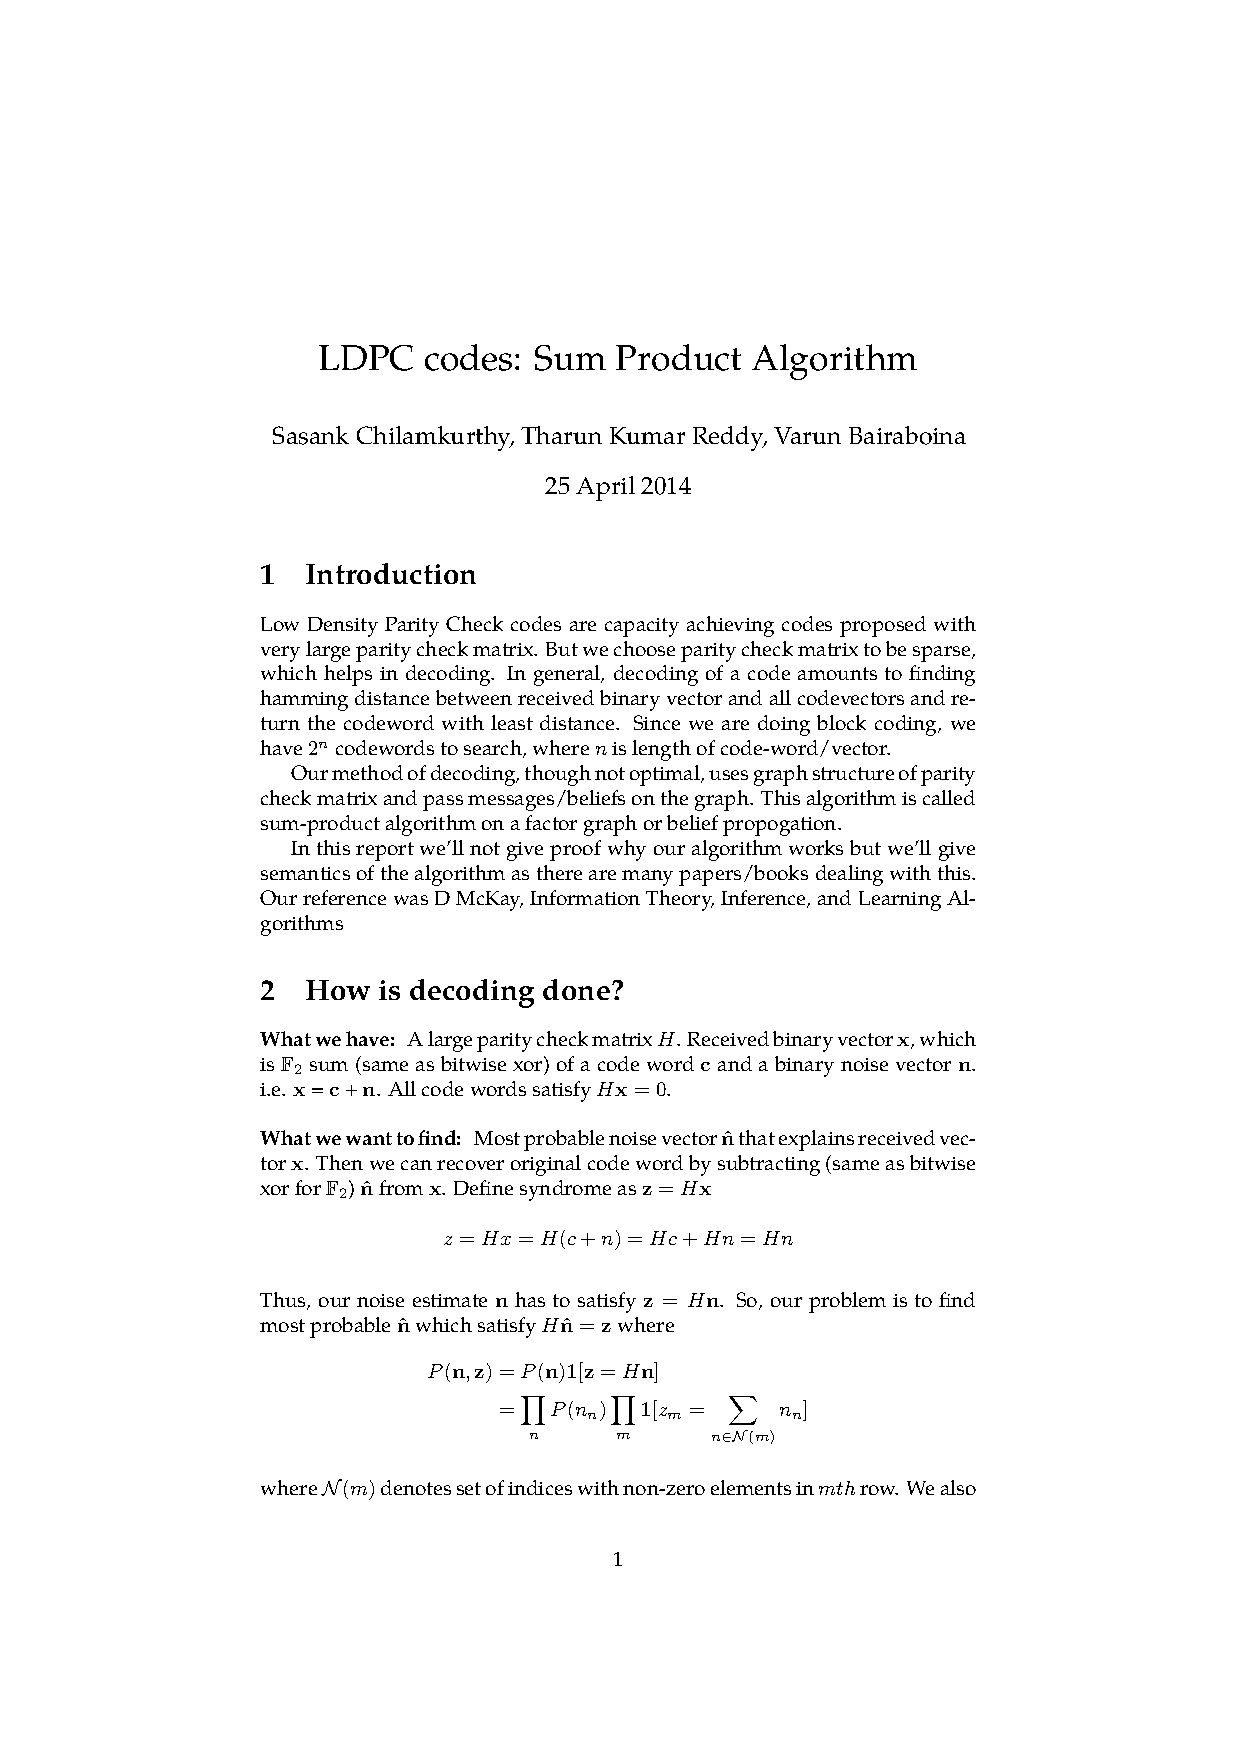
\includepdf[pages = {-}]{ldpc.pdf}
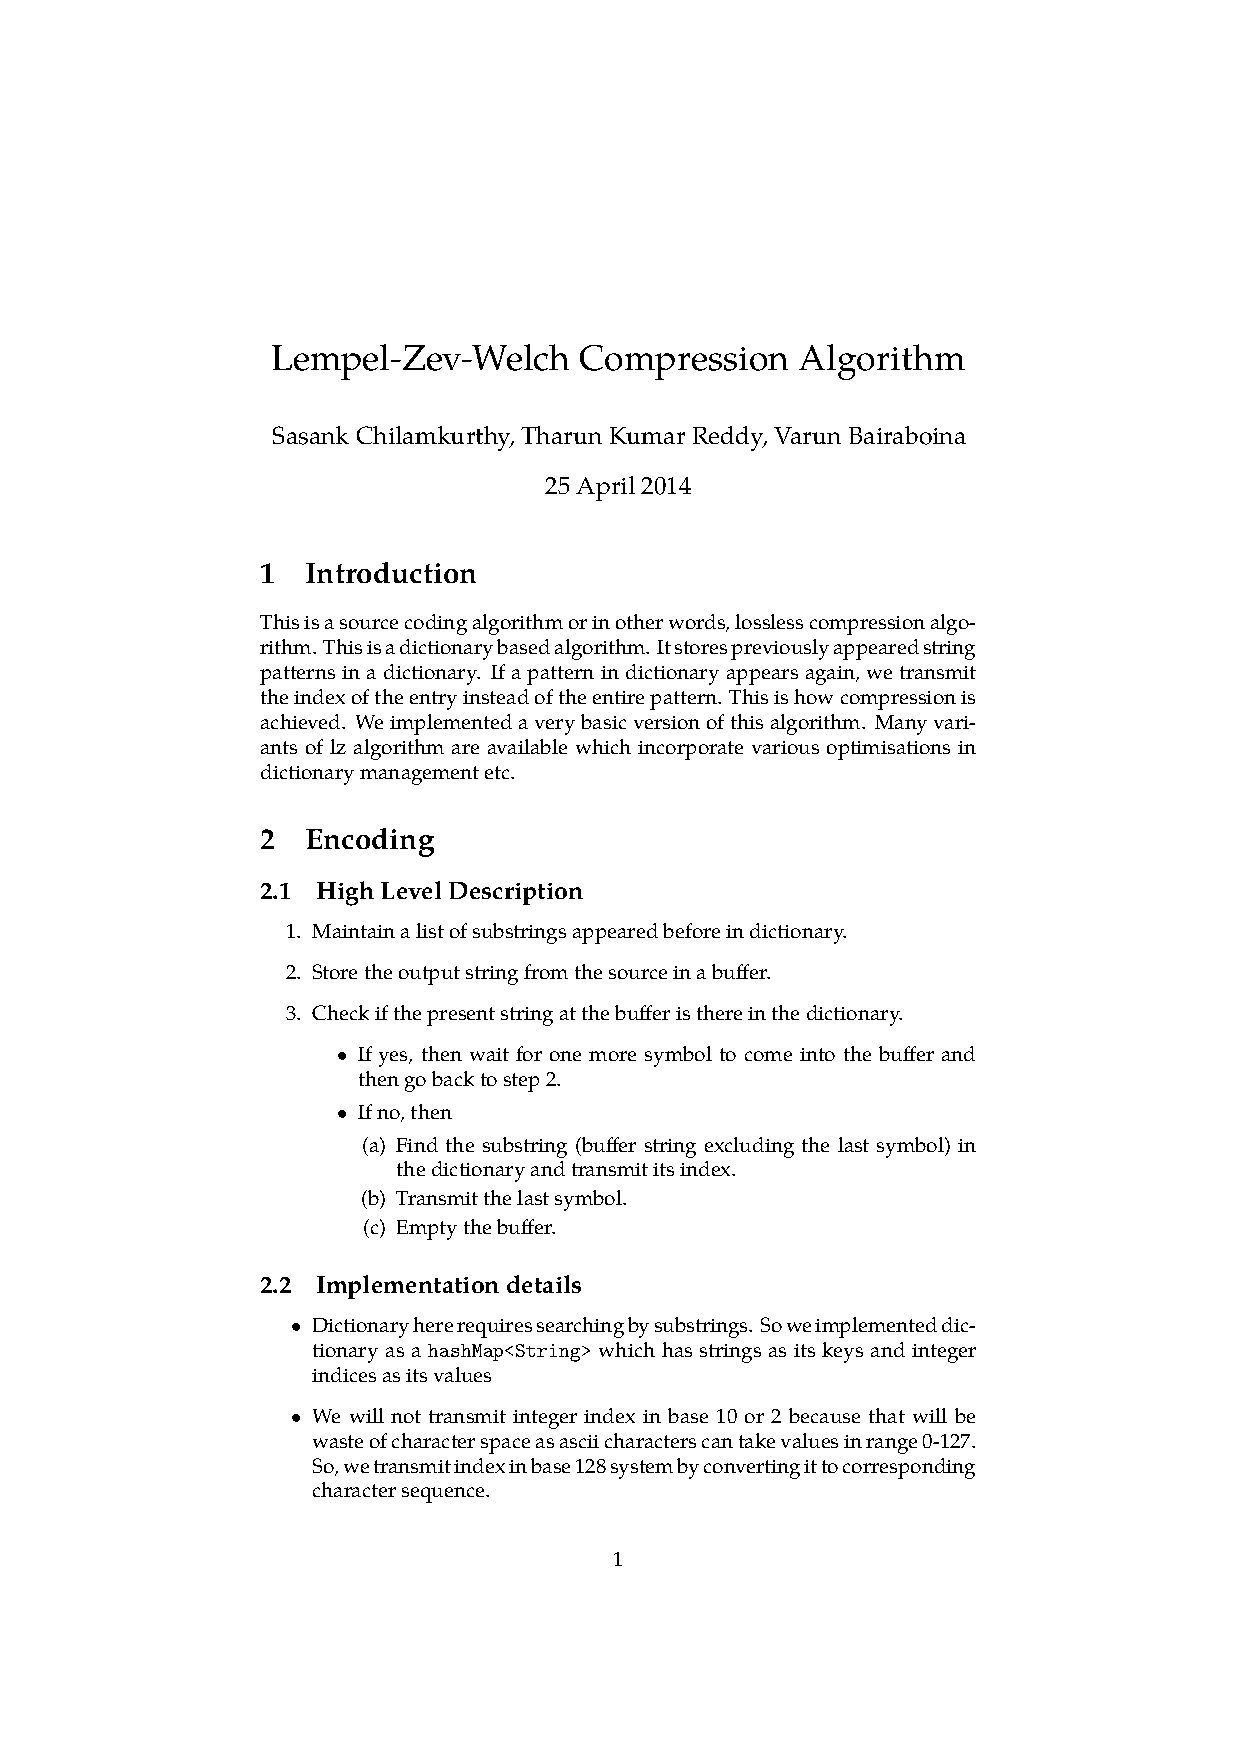
\includepdf[pages = {-}]{lwz.pdf}
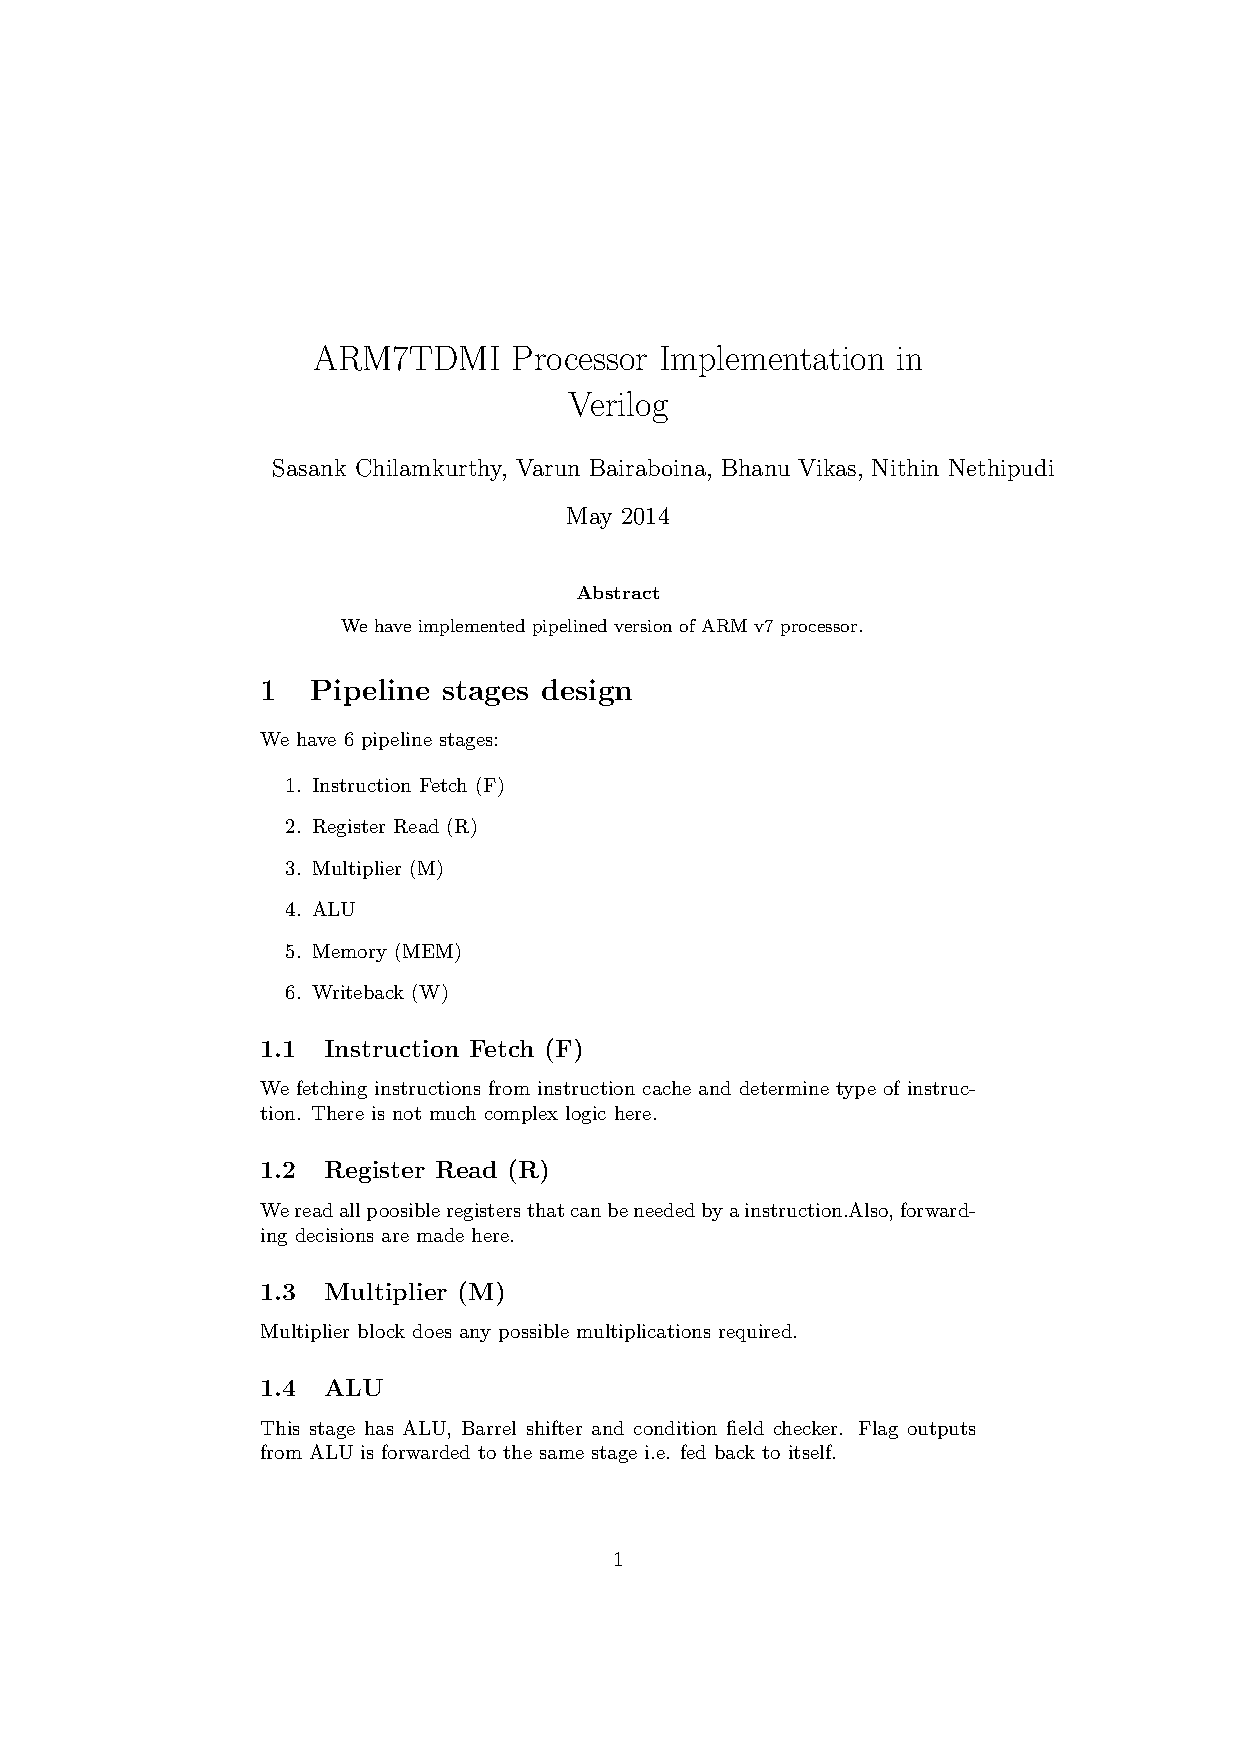
\includepdf[pages = {-}]{arm7.pdf}
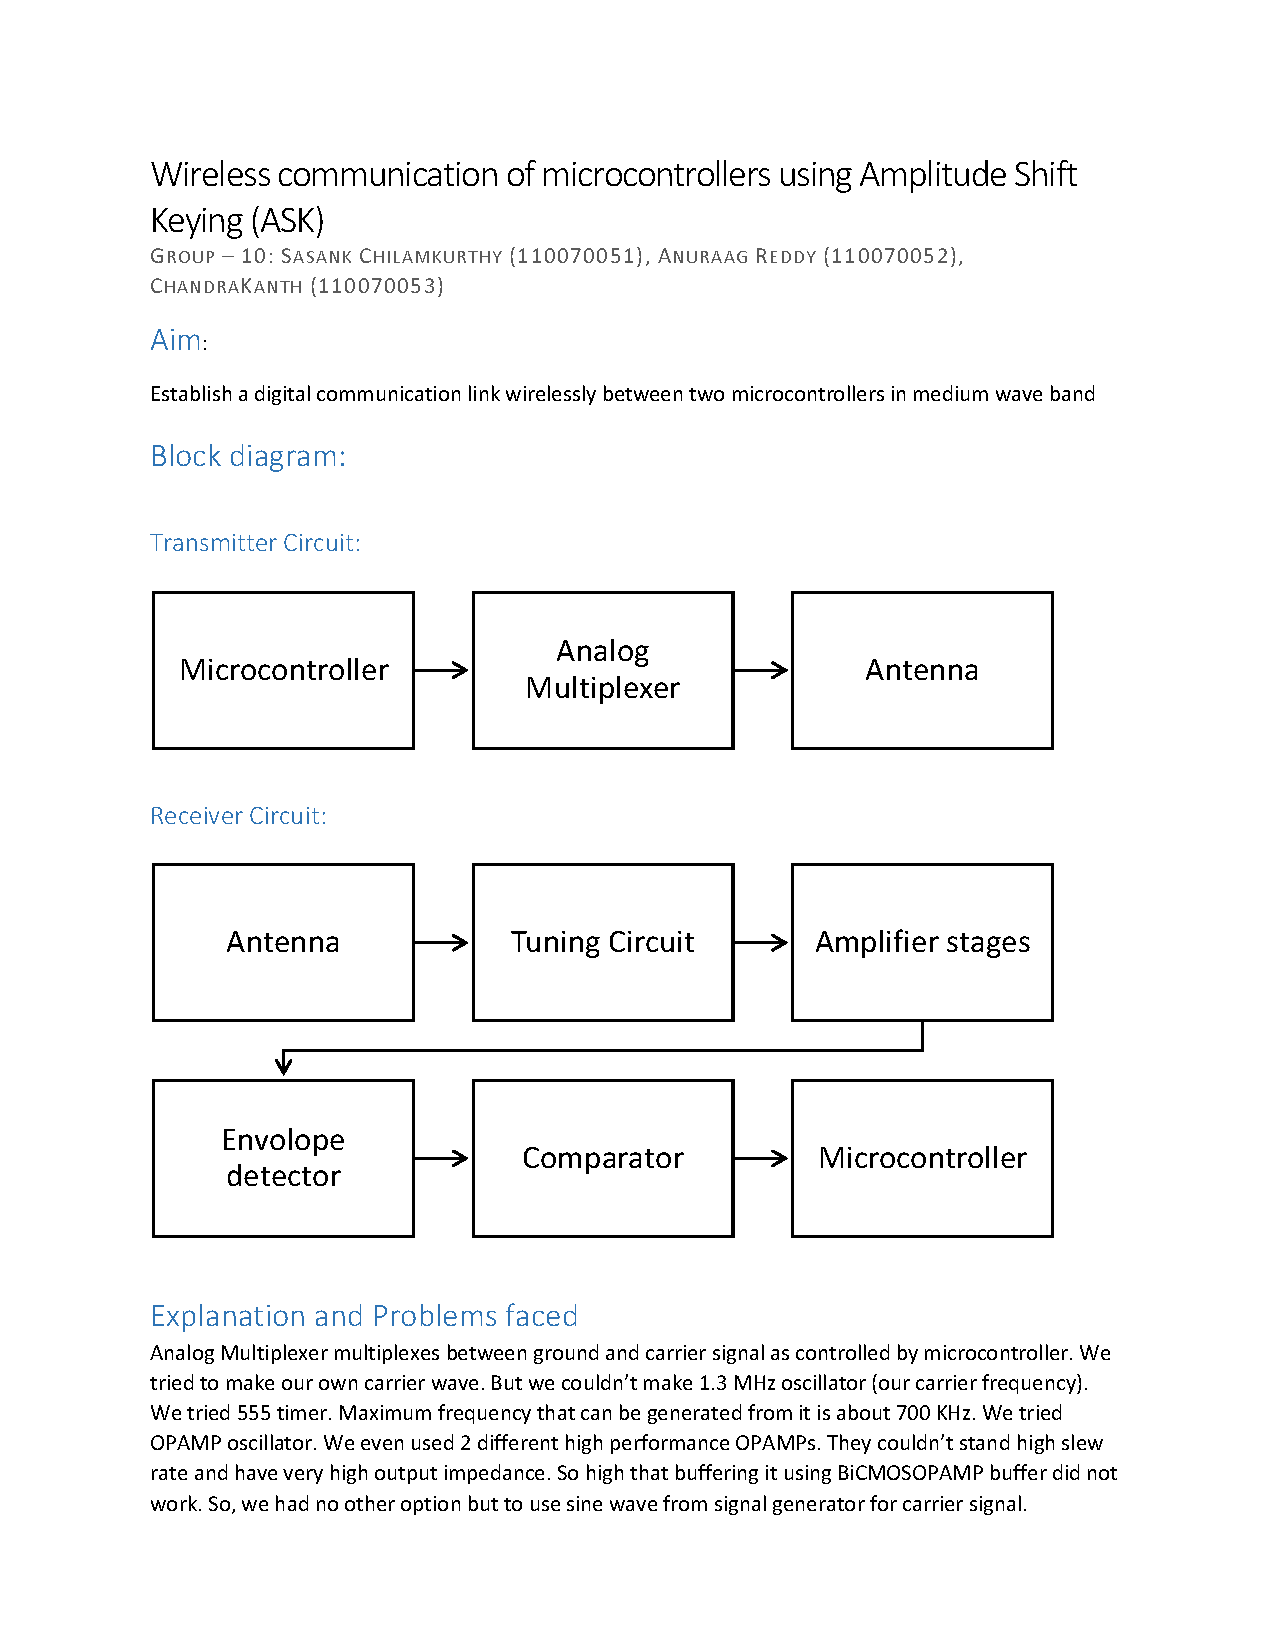
\includepdf[pages = {-}]{wireless.pdf}
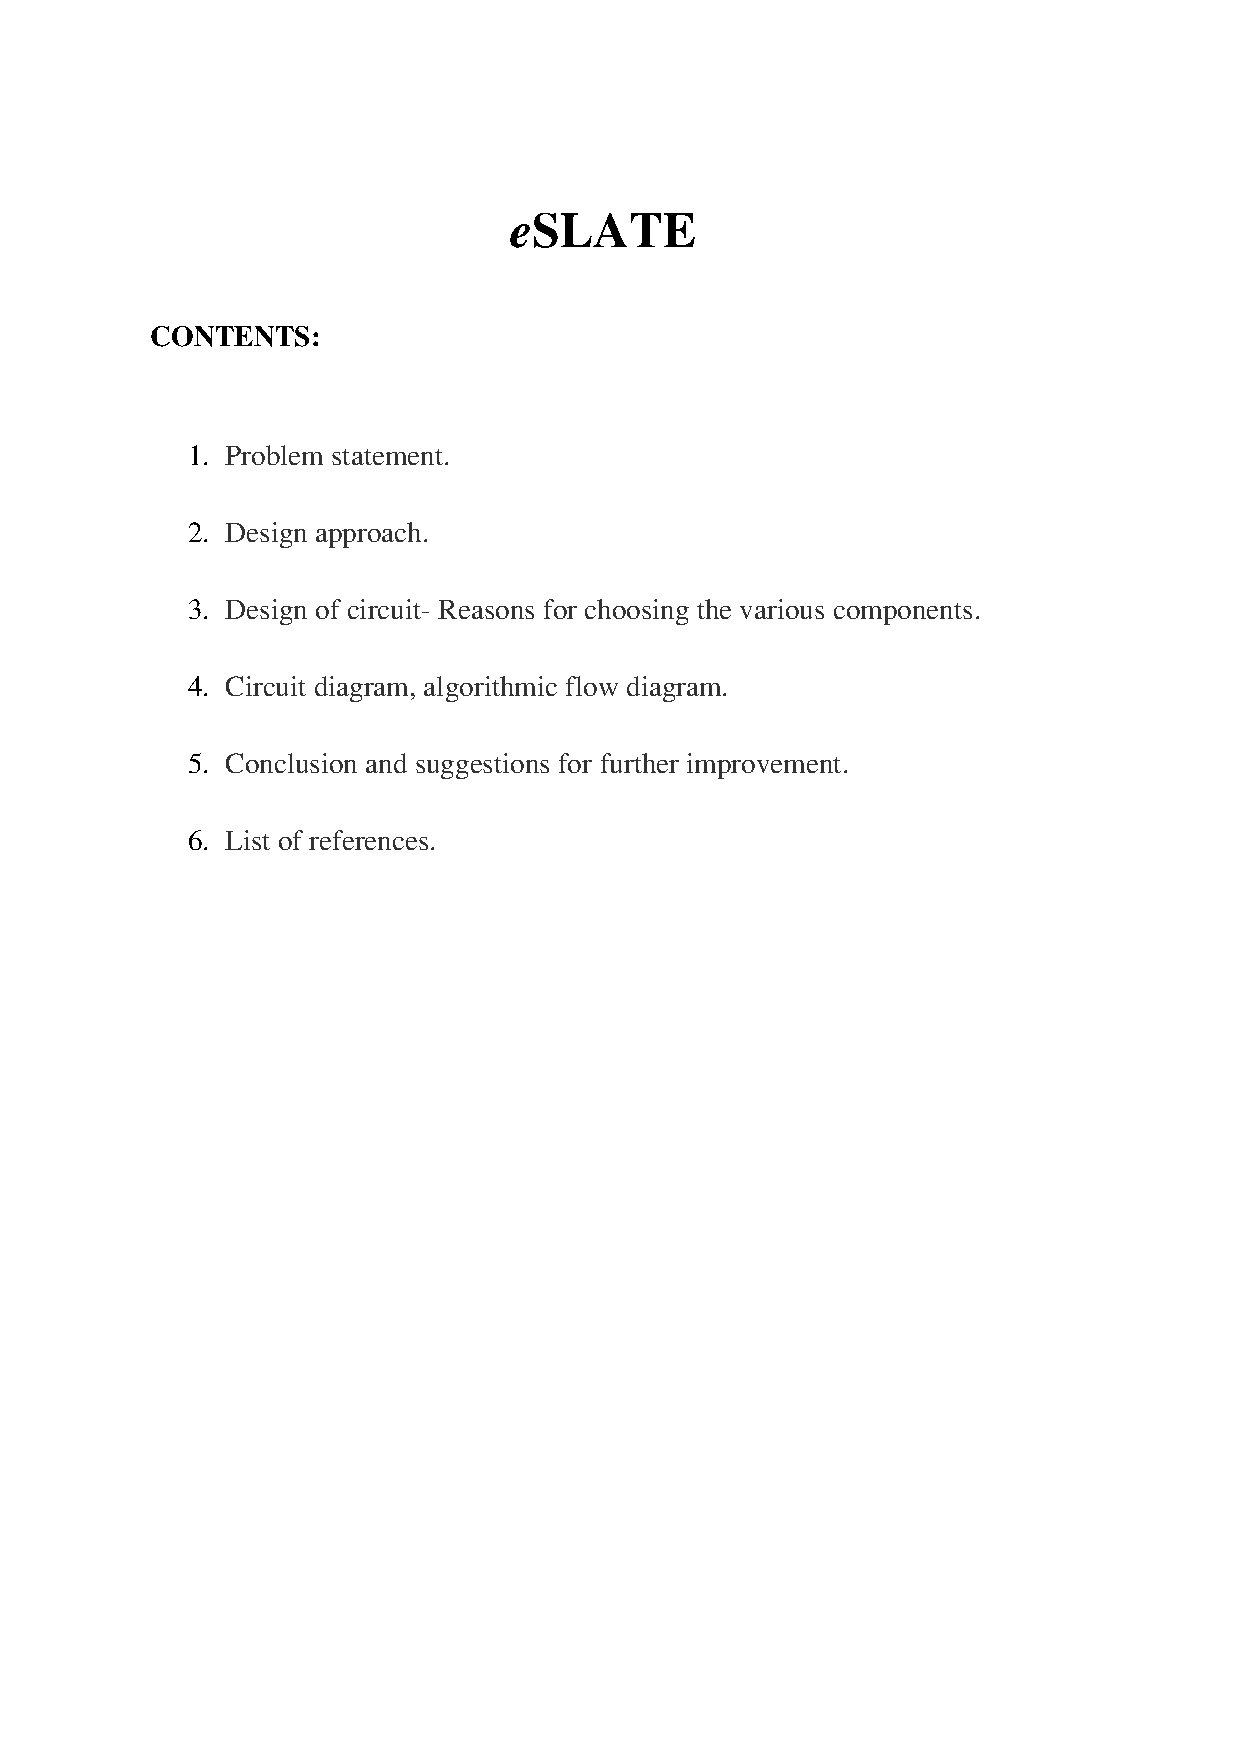
\includepdf[pages = {-}]{led_sensing.pdf}
\includepdf[pages = {-}]{dip.pdf}
\end{document}